\clearpage

\subsection{Architettura di dettaglio - Classi del sistema Monolith}\subsubsection{Check}
\textbf{Componente:}  Monolith::checks\\
   \FloatBarrier
   \begin{figure}[ht]
   \centering
   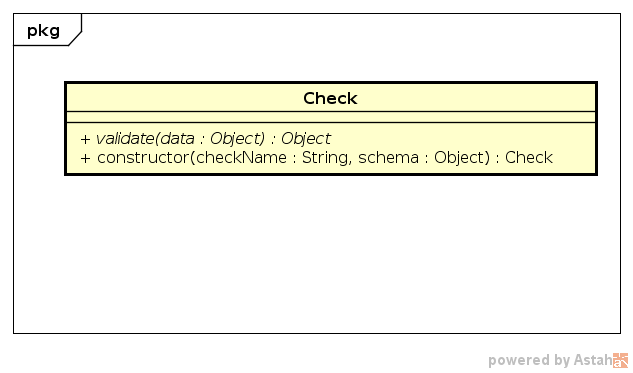
\includegraphics[width=0.6\textwidth]{img/single-Check}
   \caption{{Diagramma per Check in checks}}
\end{figure}
\FloatBarrier
\textbf{Descrizione}\\
Classe che rappresenta i controlli da eseguire lato server sull'input dell'utente. 
\\begin{itemize}
\\item +constructor(checkName: String, schema: Object) \\\\
Il costruttore riceve il nome con cui verrà registrato il controllo da eseguire e la descrizione dello schema dei dati. Il secondo argomento viene utilizzato per inizializzare un oggetto SimpleSchema.
\\item +validate(dataObj:Object):boolean \\\\
Viene controllato che l'oggetto fornito come argomento corrisponda allo schema.
\\end{itemize} 


\textbf{Applicazioni}\\
Prima di ogni inserimento sul database i dati vengono verificati utilizzando questa classe. 


\clearpage

\subsubsection{CheckHandler}
\textbf{Componente:}  Monolith::checks\\
   \FloatBarrier
   \begin{figure}[ht]
   \centering
   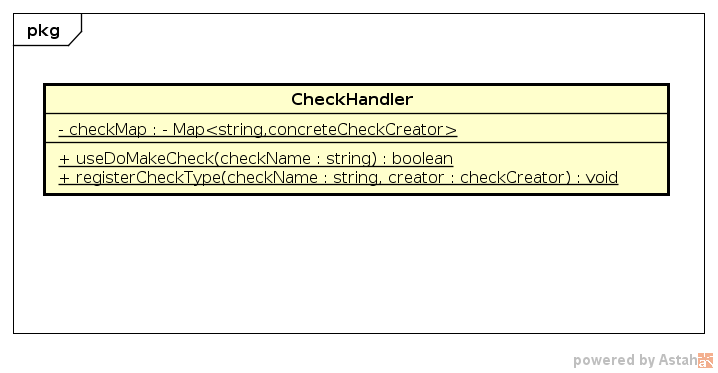
\includegraphics[width=0.6\textwidth]{img/single-CheckHandler}
   \caption{{Diagramma per CheckHandler in checks}}
\end{figure}
\FloatBarrier
\textbf{Descrizione}\\
Classe che contiene una mappa statica che associa i controlli (classe check) alle stringhe che li descrivono. 
\\begin{itemize}
\\item +registerCheck(check: Check) \\\\
Inserisce un check nella mappa
\\item +execCheck(checkName:String, dataObj: Object):boolean \\\\
Esegue il check con il nome checkName sull'oggetto dataObj e ritorna un booleano che descrive la conformità dei dati. In caso il check non sia presente nella mappa allora viene lanciato un errore.
\\end{itemize} 


\textbf{Applicazioni}\\
Viene utilizzato per eseguire i controlli sull'input lato server 


\clearpage

\subsubsection{BubbleDatabase}
\textbf{Componente:}  Monolith::Database\\
   \FloatBarrier
   \begin{figure}[ht]
   \centering
   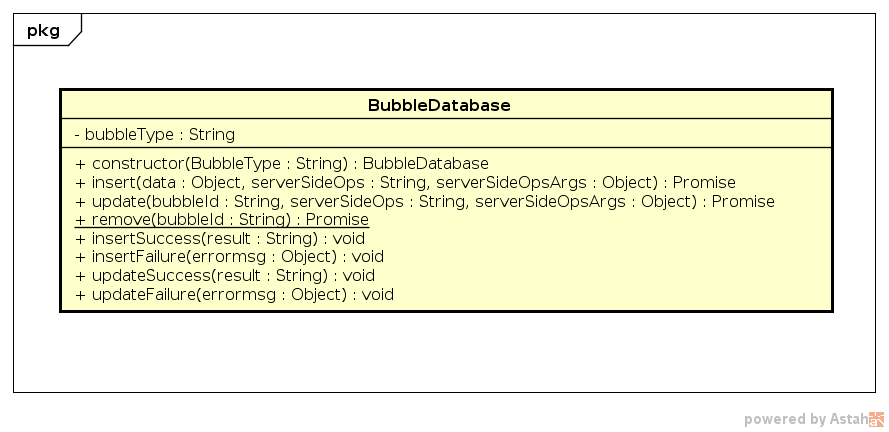
\includegraphics[width=0.6\textwidth]{img/single-BubbleDatabase}
   \caption{{Diagramma per BubbleDatabase in Database}}
\end{figure}
\FloatBarrier
\textbf{Descrizione}\\
Classe che fornisce un'interfaccia per utilizzare il database lato client. 
\\
Il costruttore chiede una stringa corrispondente al nome della bolla. Per ogni bolla si dovrà istanziare BubbleDatabase con il nome corrispondente.
\\
Ciascuno dei seguenti metodi ritorna una promise:
\\begin{itemize} 
\\item +insert(data: Object, serverSideOps, serverSideOpsArg) \\
Richiama il Meteor.Method insertBubble fornendo automaticamente alcuni parametri necessari e specificando la funzione lato server da eseguire sul database. 
\\item +update(bubbleId, serverSideOps, serverSideOpsArgs) \\
Richiama il Meteor.Method updateBubble specificando la funzione lato server da eseguire sul database.
\\item +remove(bubbleId) \\
Metodo statico che richiama il Meteor.method per rimuovere la bolla con l'id passato come agomento
\\end{itemize}
I restanti metodi (insertSuccess, insertFailure, updateSuccess, updateFailure) vengono invocati automaticamente al successo o al fallimento di una delle operazioni sopra descritte e semplicemente stampano un messaggio sulla console. In caso di necessità possono essere ridefinite derivando la classe. 


\textbf{Applicazioni}\\
 


\clearpage

\subsubsection{SideArea1}
\textbf{Componente:}  Monolith::SideAreas::SideArea1\_pkg\\
   \FloatBarrier
   \begin{figure}[ht]
   \centering
   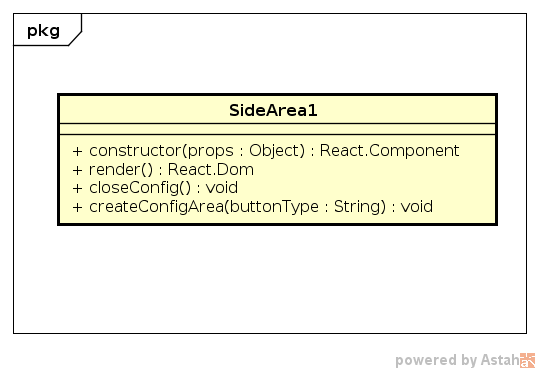
\includegraphics[width=0.6\textwidth]{img/single-SideArea1}
   \caption{{Diagramma per SideArea1 in SideArea1\_pkg}}
\end{figure}
\FloatBarrier
\textbf{Descrizione}\\
Classe che rappresenta il componente React per la visualizzazione del contenuto della prima area laterale. \\\\ 
\\textbf{Metodi:}
\\begin{itemize}

\\item +constructor(props : Object) : React.Component 
\\\\
Costruttore della sottoclasse di React.Component in cui è necessario chiamare super (props) ed è possibile inizializzare lo stato per i dati soggetti a cambiamento.

\\item +render() : React.DOM 
\\\\
Metodo che esamina this.props e this.state e restituisce un componente che funga da contenitore per la prima area laterale.

\\end{itemize} 


\textbf{Applicazioni}\\
Viene utilizzata all'apertura della prima area laterale per visualizzare il menù di creazione delle bolle e lo storico delle bolle inviate. 


\clearpage

\subsubsection{BubbleMenu}
\textbf{Componente:}  Monolith::SideAreas::SideArea1\_pkg\\
   \FloatBarrier
   \begin{figure}[ht]
   \centering
   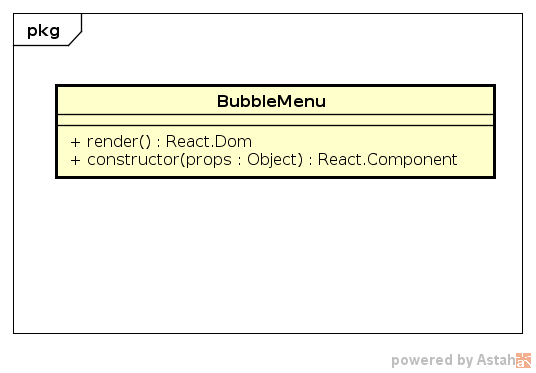
\includegraphics[width=0.6\textwidth]{img/single-BubbleMenu}
   \caption{{Diagramma per BubbleMenu in SideArea1\_pkg}}
\end{figure}
\FloatBarrier
\textbf{Descrizione}\\
Classe che contiene i pulsanti che portano alla configurazione delle singole bolle.
\\textbf{Metodi:} 
\\begin{itemize}
\\item +constructor(props : Object) : React.Component 
\\\\
Costruttore della sottoclasse di React.Component in cui è necessario chiamare super (props) ed è possibile inizializzare lo stato per i dati soggetti a cambiamento.
\\item +render() : React.DOM 
\\\\
Metodo che esamina this.props e this.state e restituisce un singolo elemento React che può essere una rappresentazione di un componente DOM nativo o un altro componente composito.
\\end{itemize} 


\textbf{Applicazioni}\\
Viene utilizzata dalla SideArea1 per la visualizzazione del menù contenente i pulsanti per la creazione delle bolle. 


\clearpage

\subsubsection{ConfigArea}
\textbf{Componente:}  Monolith::SideAreas::SideArea1\_pkg\\
   \FloatBarrier
   \begin{figure}[ht]
   \centering
   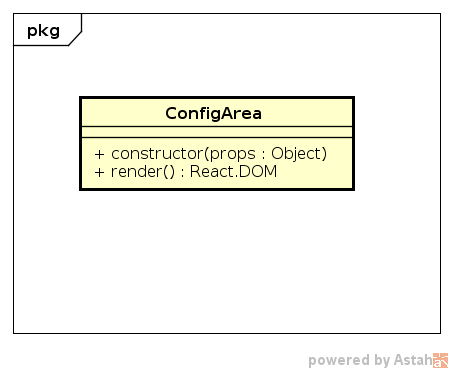
\includegraphics[width=0.6\textwidth]{img/single-ConfigArea}
   \caption{{Diagramma per ConfigArea in SideArea1\_pkg}}
\end{figure}
\FloatBarrier
\textbf{Descrizione}\\
Componente React in cui la SideArea1 inserisce i componenti grafici di configurazione. Questi possono essere i menu di configurazione per le bolle o altri menu di impostazioni 


\textbf{Applicazioni}\\
Viene utilizzato da SideArea1 per mostrare componenti grafici a scomparsa 


\clearpage

\subsubsection{SentBubbles}
\textbf{Componente:}  Monolith::SideAreas::SideArea1\_pkg\\
   \FloatBarrier
   \begin{figure}[ht]
   \centering
   \includegraphics[width=0.6\textwidth]{img/single-SentBubbles}
   \caption{{Diagramma per SentBubbles in SideArea1\_pkg}}
\end{figure}
\FloatBarrier
\textbf{Descrizione}\\
Classe che rappresenta il componente React per la visualizzazione dello storico delle bolle inviate.

\\textbf{Metodi:} 
\\begin{itemize}

\\item +constructor(props : Object) : React.Component 
\\\\
Costruttore della sottoclasse di React.Component in cui è necessario chiamare super (props) ed è possibile inizializzare lo stato per i dati soggetti a cambiamento.

\\item +render() : React.DOM 
\\\\
Metodo che esamina this.props e this.state e restituisce un componente che raccolga lo storico delle bolle inviate.

\\end{itemize} 


\textbf{Applicazioni}\\
Viene utilizzata dalla SideArea1 per la visualizzazione dello storico delle bolle inviate. 


\clearpage

\subsubsection{SideArea2}
\textbf{Componente:}  Monolith::SideAreas::SideArea2\_pkg\\
   \FloatBarrier
   \begin{figure}[ht]
   \centering
   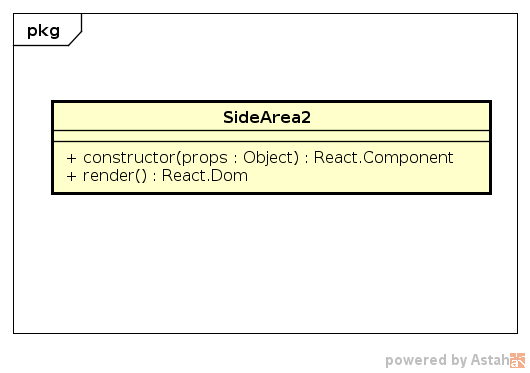
\includegraphics[width=0.6\textwidth]{img/single-SideArea2}
   \caption{{Diagramma per SideArea2 in SideArea2\_pkg}}
\end{figure}
\FloatBarrier
\textbf{Descrizione}\\
Classe che rappresenta il componente React per la visualizzazione del contenuto della seconda area laterale. \\\\
\\textbf{Metodi:} 
\\begin{itemize}

\\item +constructor(props : Object) : React.Component 
\\\\
Costruttore della sottoclasse di React.Component in cui è necessario chiamare super (props) ed è possibile inizializzare lo stato per i dati soggetti a cambiamento.

\\item +render() : React.DOM 
\\\\
Metodo che esamina this.props e this.state e restituisce un componente che funge da contenitore per la seconda area laterale.

\\end{itemize} 


\textbf{Applicazioni}\\
Viene utilizzata all'apertura della seconda area laterale per visualizzare dello storico delle bolle ricevute. 


\clearpage

\subsubsection{ReceivedBubble}
\textbf{Componente:}  Monolith::SideAreas::SideArea2\_pkg\\
   \FloatBarrier
   \begin{figure}[ht]
   \centering
   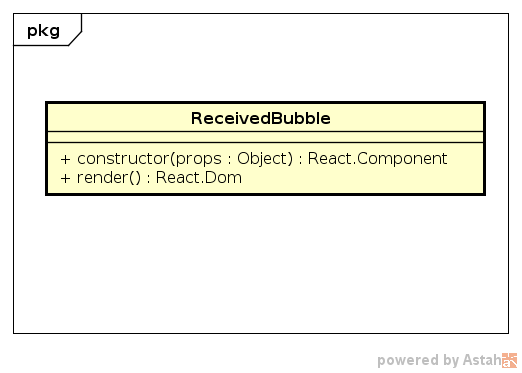
\includegraphics[width=0.6\textwidth]{img/single-ReceivedBubble}
   \caption{{Diagramma per ReceivedBubble in SideArea2\_pkg}}
\end{figure}
\FloatBarrier
\textbf{Descrizione}\\
Classe che rappresenta il componente React per la visualizzazione dello storico delle bolle ricevute. \\\\
\\textbf{Metodi:} 
\\begin{itemize}
\\item +constructor(props : Object) : React.Component 
\\\\
Costruttore della sottoclasse di React.Component in cui è necessario chiamare super (props) ed è possibile inizializzare lo stato per i dati soggetti a cambiamento.
\\item +render() : React.DOM 
\\\\
Metodo che esamina this.props e this.state e restituisce un singolo elemento React che può essere una rappresentazione di un componente DOM nativo o un altro componente composito.
\\end{itemize} 


\textbf{Applicazioni}\\
Viene utilizzata dalla SideArea2 per la visualizzazione dello storico delle bolle ricevute. 


\clearpage

\subsubsection{VerticalLayout}
\textbf{Componente:}  Monolith::UI::Layouts\\
   \FloatBarrier
   \begin{figure}[ht]
   \centering
   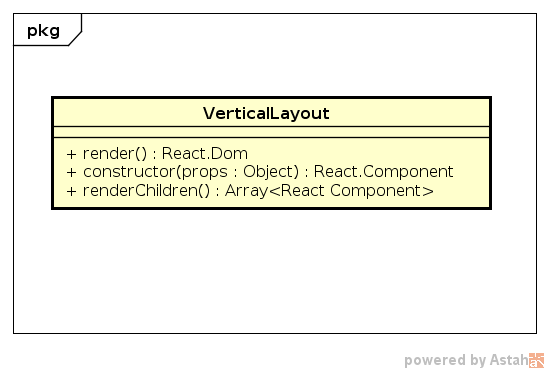
\includegraphics[width=0.6\textwidth]{img/single-VerticalLayout}
   \caption{{Diagramma per VerticalLayout in Layouts}}
\end{figure}
\FloatBarrier
\textbf{Descrizione}\\
Classe contenitore che dispone i componenti contenuti in verticale. \\\\
\\textbf{Metodi:}
\\begin{itemize}

\\item +constructor(props : Object) : React.Component 
\\\\
Costruttore della sottoclasse di React.Component in cui è necessario chiamare super (props) ed è possibile inizializzare lo stato per i dati soggetti a cambiamento.

\\item +render() : React.DOM 
\\\\
Metodo che esamina this.props e this.state e restituisce un contenitore di elementi che li dispone in verticale.

\\item +countMyChildren() : int
\\\\
Metodo che ritorna un intero contente il numero di componenti figli, utilizzato per impostare la classe bootstrap corretta.

\\end{itemize} 


\textbf{Applicazioni}\\
Utilizzata per assegnare l'attributo className bootstrap a tutti i componenti figli, in modo che vengano visualizzati allineati in verticale con la dimensione adeguata. 


\clearpage

\subsubsection{ContainedElement}
\textbf{Componente:}  Monolith::UI::Layouts\\
   \FloatBarrier
   \begin{figure}[ht]
   \centering
   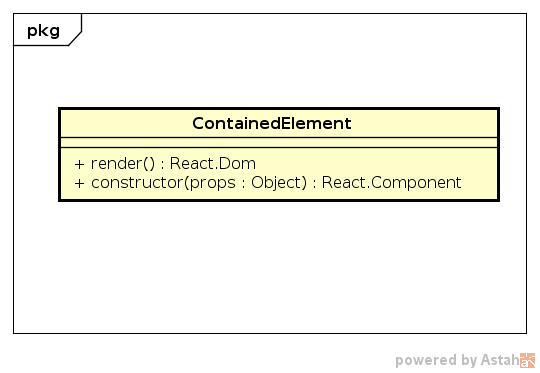
\includegraphics[width=0.6\textwidth]{img/single-ContainedElement}
   \caption{{Diagramma per ContainedElement in Layouts}}
\end{figure}
\FloatBarrier
\textbf{Descrizione}\\
Classe che rappresenta il layout di un contenitore generico. \\\\
\\textbf{Metodi:} 
\\begin{itemize}

\\item +constructor(props : Object) : React.Component 
\\\\
Costruttore della sottoclasse di React.Component in cui è necessario chiamare super (props) ed è possibile inizializzare lo stato per i dati soggetti a cambiamento.

\\item +render() : React.DOM 
\\\\
Metodo che esamina this.props e this.state e restituisce un elemento "div" contenenti i figli ed utilizzando lo stile CSS passato nella props "classNames".

\\end{itemize} 


\textbf{Applicazioni}\\
Viene utilizzata dalle classi HorizontalLayout, VerticalLayout e ConditionalRendering per contenere un componente generico 


\clearpage

\subsubsection{HorizontalLayout}
\textbf{Componente:}  Monolith::UI::Layouts\\
   \FloatBarrier
   \begin{figure}[ht]
   \centering
   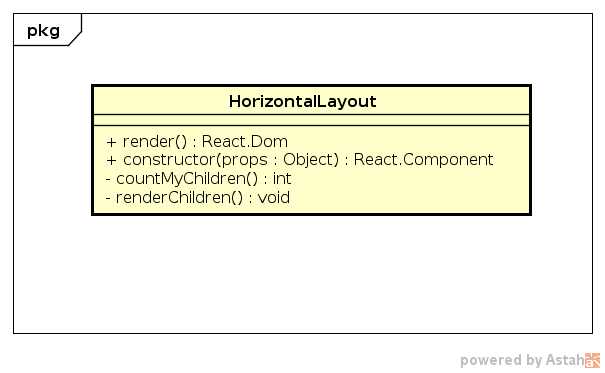
\includegraphics[width=0.6\textwidth]{img/single-HorizontalLayout}
   \caption{{Diagramma per HorizontalLayout in Layouts}}
\end{figure}
\FloatBarrier
\textbf{Descrizione}\\
Classe contenitore che dispone i componenti contenuti in orizzontale. \\\\
\\textbf{Metodi:}
\\begin{itemize}

\\item +constructor(props : Object) : React.Component 
\\\\
Costruttore della sottoclasse di React.Component in cui è necessario chiamare super (props) ed è possibile inizializzare lo stato per i dati soggetti a cambiamento.

\\item +render() : React.DOM 
\\\\
Metodo che esamina this.props e this.state e restituisce un contenitore di elementi che li dispone in orizzontale.

\\item +countMyChildren() : int \\\\
Metodo che ritorna un intero contente il numero di componenti figli, utilizzato per impostare la classe bootstrap corretta.

\\end{itemize} 


\textbf{Applicazioni}\\
Utilizzata per assegnare l'attributo className bootstrap a tutti i componenti figli, in modo che vengano visualizzati allineati in orizzontale con la dimensione adeguata. 


\clearpage

\subsubsection{Image}
\textbf{Componente:}  Monolith::UI::SingleComponents\\
   \FloatBarrier
   \begin{figure}[ht]
   \centering
   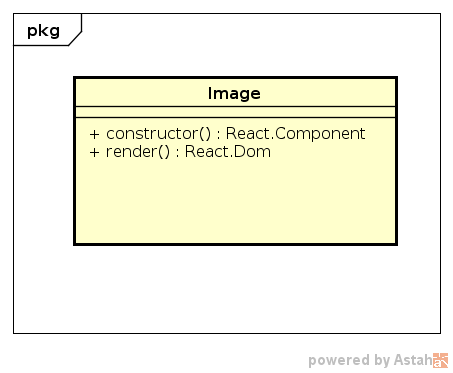
\includegraphics[width=0.6\textwidth]{img/single-Image}
   \caption{{Diagramma per Image in SingleComponents}}
\end{figure}
\FloatBarrier
\textbf{Descrizione}\\
Componente React che rappresenta un'immagine. \\\\
\\textbf{Metodi:} 
\\begin{itemize}
\\item +constructor(props : Object) : React.Component 
\\\\
Costruttore della sottoclasse di React.Component in cui è necessario chiamare super (props) ed è possibile inizializzare lo stato per i dati soggetti a cambiamento.
\\item +render() : React.DOM 
\\\\
Metodo che esamina this.props e this.state e restituisce un immagine con le proprietà datele.
\\end{itemize} 


\textbf{Applicazioni}\\
Viene utilizzato per rappresentare un immagine all'interno di una bolla.
Image può avere le seguenti props:
\\begin{itemize}
\\item classes:
\\\\
Stile CSS per il componente.
\\item id:
\\\\
Un Id per il componente React.
\\item src: 
\\\\
Come per tag HTML "img".
\\item alt: 
\\\\
Come per tag HTML "img".
\\item width: \\\\
Come per tag HTML "img".
\\item height: \\\\
Come per tag HTML "img". 


\clearpage

\subsubsection{ComboBox}
\textbf{Componente:}  Monolith::UI::SingleComponents\\
   \FloatBarrier
   \begin{figure}[ht]
   \centering
   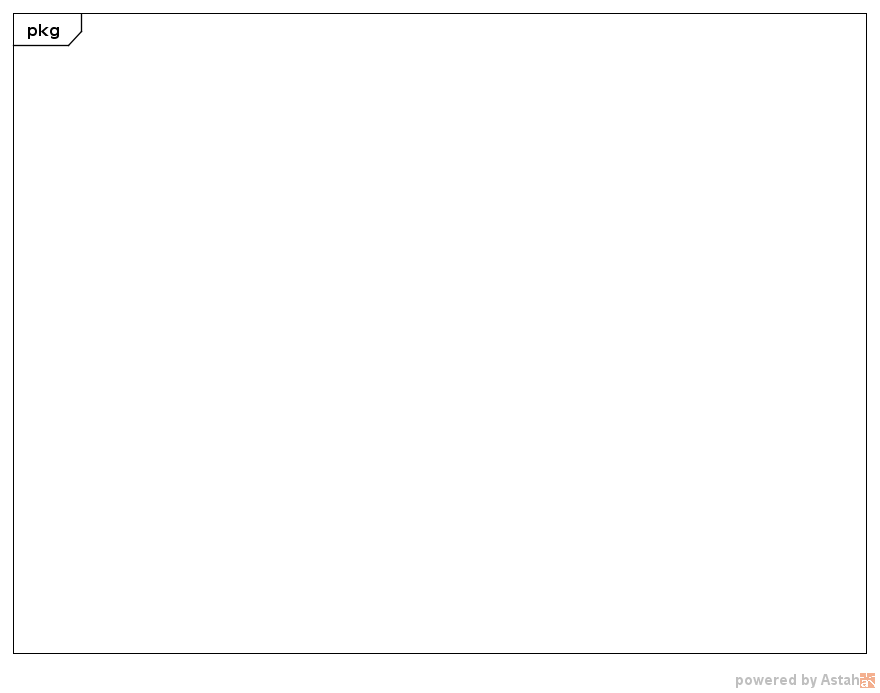
\includegraphics[width=0.6\textwidth]{img/single-ComboBox}
   \caption{{Diagramma per ComboBox in SingleComponents}}
\end{figure}
\FloatBarrier
\textbf{Descrizione}\\
Componente React che rappresenta un combobox. \\\\
\\textbf{Metodi:} 
\\begin{itemize}
\\item +constructor(props : Object) : React.Component 
\\\\
Costruttore della sottoclasse di React.Component in cui è necessario chiamare super (props) ed è possibile inizializzare lo stato per i dati soggetti a cambiamento.

\\item +optChange(event : String) : void  
\\\\
Comunica alla funzione "padre" l'opzione selezionata.

\\item +render() : React.DOM 
\\\\
Metodo che esamina this.props e this.state e restituisce un singolo elemento combobox con le opzione passategli nelle props.

\\end{itemize} 


\textbf{Applicazioni}\\
Componente React rappresentante una combobox e costruibile passando un array contenente le varie opzioni nella props "options". 


\clearpage

\subsubsection{LineEdit}
\textbf{Componente:}  Monolith::UI::SingleComponents\\
   \FloatBarrier
   \begin{figure}[ht]
   \centering
   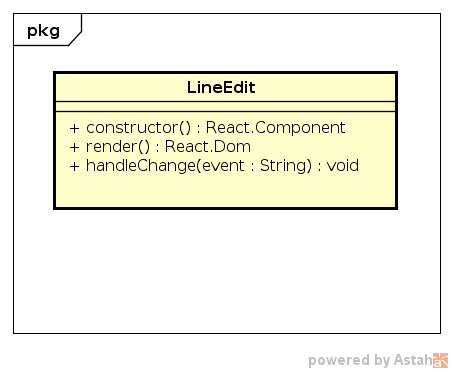
\includegraphics[width=0.6\textwidth]{img/single-LineEdit}
   \caption{{Diagramma per LineEdit in SingleComponents}}
\end{figure}
\FloatBarrier
\textbf{Descrizione}\\
Componente React che rappresenta un input di testo. \\\\
\\textbf{Metodi:} 
\\begin{itemize}
\\item +constructor(props : Object) : React.Component 
\\\\
Costruttore della sottoclasse di React.Component in cui è necessario chiamare super (props) ed è possibile inizializzare lo stato per i dati soggetti a cambiamento.
\\item +handleChange(event : String) : void  
\\\\
Comunica la stringa digitata al "padre". 
\\item +render() : React.DOM 
\\\\
Metodo che esamina this.props e this.state e restituisce un singolo elemento React che rappresenta un input di testo.
\\end{itemize} 


\textbf{Applicazioni}\\
Viene utilizzato per costruire eventuali interfacce grafiche delle bolle. \\\\
Si aspetta una props "id" per distinguere il componente. 


\clearpage

\subsubsection{PushButton}
\textbf{Componente:}  Monolith::UI::SingleComponents\\
   \FloatBarrier
   \begin{figure}[ht]
   \centering
   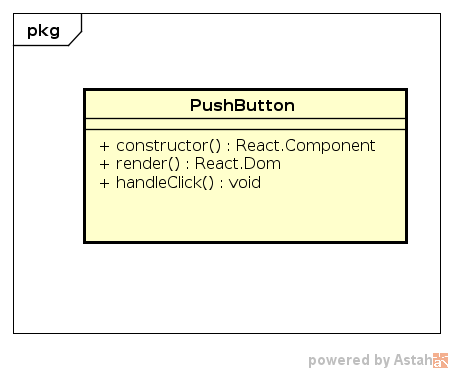
\includegraphics[width=0.6\textwidth]{img/single-PushButton}
   \caption{{Diagramma per PushButton in SingleComponents}}
\end{figure}
\FloatBarrier
\textbf{Descrizione}\\
Componente React che rappresenta un pulsante. \\\\
\\textbf{Metodi:} 
\\begin{itemize}
\\item +constructor(props : Object) : React.Component 
\\\\
Costruttore della sottoclasse di React.Component in cui è necessario chiamare super (props) ed è possibile inizializzare lo stato per i dati soggetti a cambiamento.

\\item +onClick(): void 
\\\\ 
Viene passato al "padre" l'ID del pulsante cliccato.

\\item +render() : React.DOM 
\\\\
Metodo che esamina this.props e this.state e restituisce un singolo elemento React che rappresenta un pulsante eventualmente cliccabile.

\\end{itemize} 


\textbf{Applicazioni}\\
Componente React che rappresenta un pulsante che può essere cliccabile (o meno) in base all valore della props "dis". \\\\ Questa può assumere valore \\textit{true} o \\textit{false}. 


\clearpage

\subsubsection{CheckButton}
\textbf{Componente:}  Monolith::UI::SingleComponents\\
   \FloatBarrier
   \begin{figure}[ht]
   \centering
   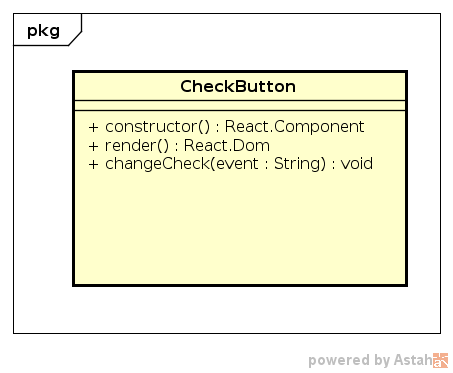
\includegraphics[width=0.6\textwidth]{img/single-CheckButton}
   \caption{{Diagramma per CheckButton in SingleComponents}}
\end{figure}
\FloatBarrier
\textbf{Descrizione}\\
Componente React che rappresenta un elemento di checkbox. \\\\
\\textbf{Metodi:} 
\\begin{itemize}

\\item +constructor(props : Object) : React.Component 
\\\\
Costruttore della sottoclasse di React.Component in cui è necessario chiamare super (props) ed è possibile inizializzare lo stato per i dati soggetti a cambiamento.

\\item +changeCheck(event : String) : void  
\\\\
Comunica l’opzione selezionata tramite il metodo del genitore. 

\\item +render() : React.DOM 
\\\\
Metodo che esamina this.props e this.state e restituisce un singolo elemento React che può essere una rappresentazione di un componente DOM nativo o un altro componente composito.

\\end{itemize} 


\textbf{Applicazioni}\\
Componente React che rappresenta un checkbox e contiene un metodo per comunicare al "padre" tutti i dati del oggetto quando questo viene cliccato. 


\clearpage

\subsubsection{ImageButton}
\textbf{Componente:}  Monolith::UI::SingleComponents\\
   \FloatBarrier
   \begin{figure}[ht]
   \centering
   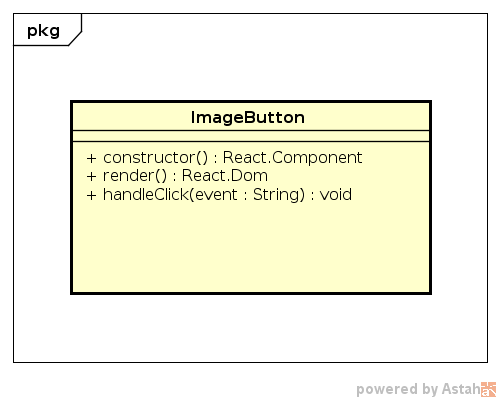
\includegraphics[width=0.6\textwidth]{img/single-ImageButton}
   \caption{{Diagramma per ImageButton in SingleComponents}}
\end{figure}
\FloatBarrier
\textbf{Descrizione}\\
Componente React che rappresenta un immagine che funge da pulsante. \\\\
\\textbf{Metodi:} 
\\begin{itemize}
\\item +constructor(props : Object) : React.Component 
\\\\
Costruttore della sottoclasse di React.Component in cui è necessario chiamare super (props) ed è possibile inizializzare lo stato per i dati soggetti a cambiamento.
\\item +handleClick() : void 
\\\\
Comunica l'Id dell'immagine cliccata al "padre". 
\\item +render() : React.DOM 
\\\\
Metodo che esamina this.props e this.state e restituisce un singolo elemento React che rappresenta un'immagine cliccabile.
\\end{itemize} 


\textbf{Applicazioni}\\
Componente React che rappresenta un'immagine cliccabile.\\\\ Richiede le stesse props del componente "Image" con l'aggiunta di "handleClick" che comunica al "padre" l'id del componente cliccato. 


\clearpage

\subsubsection{CheckBoxList}
\textbf{Componente:}  Monolith::UI::SingleComponents\\
   \FloatBarrier
   \begin{figure}[ht]
   \centering
   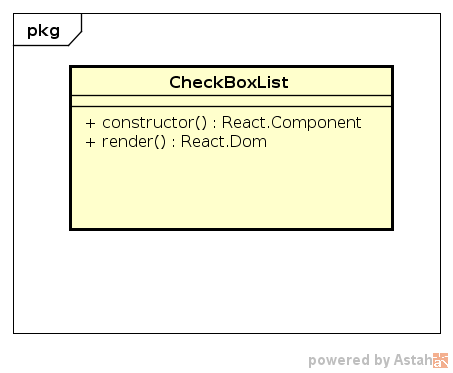
\includegraphics[width=0.6\textwidth]{img/single-CheckBoxList}
   \caption{{Diagramma per CheckBoxList in SingleComponents}}
\end{figure}
\FloatBarrier
\textbf{Descrizione}\\
Componente React che rappresenta una lista di CheckButton. \\\\
\\textbf{Metodi:} 
\\begin{itemize}
\\item +constructor(props : Object) : React.Component 
\\\\
Costruttore della sottoclasse di React.Component in cui è necessario chiamare super (props) ed è possibile inizializzare lo stato per i dati soggetti a cambiamento.

\\item +getCheck (n : Object) : void \\\\
Funzione che passa al "padre" i dati del CheckButton cliccato. 

\\item +render() : React.DOM 
\\\\
Metodo che esamina this.props e this.state e restituisce un singolo elemento React che può essere una rappresentazione di un componente DOM nativo o un altro componente composito.

\\end{itemize}
\\\\
\\textbf{Props:} 
\\begin{itemize}
\\item options: 
\\\\
Passare un array di opzioni contenenti, per ciascuna di esse, un "id" ed un "value".
\\item getCheck: 
\\\\
Passare una funzione che raccolga un oggetto di ritorno contenente i dati del CheckButton cliccato.

\\end{itemize} 


\textbf{Applicazioni}\\
Componente React utile per costruire una lista di CheckButton passandogli un array di opzioni. 


\clearpage

\subsubsection{TextAreaButton}
\textbf{Componente:}  Monolith::UI::SingleComponents\\
   \FloatBarrier
   \begin{figure}[ht]
   \centering
   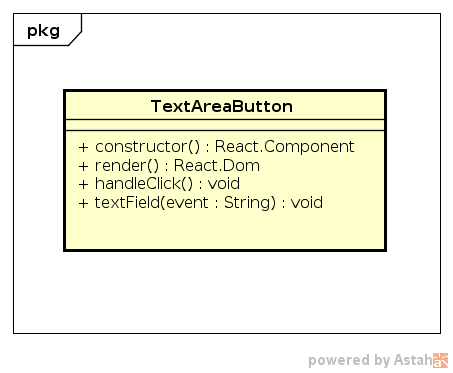
\includegraphics[width=0.6\textwidth]{img/single-TextAreaButton}
   \caption{{Diagramma per TextAreaButton in SingleComponents}}
\end{figure}
\FloatBarrier
\textbf{Descrizione}\\
Componente React che rappresenta un'area di testo con un pulsante. \\\\
\\textbf{Metodi:} 
\\begin{itemize}

\\item +constructor(props : Object) : React.Component 
\\\\
Costruttore della sottoclasse di React.Component in cui è necessario chiamare super (props) ed è possibile inizializzare lo stato per i dati soggetti a cambiamento.

\\item +textField(text : String) : void 
\\\\
Salva il testo scritto nella TextArea.

\\item +handleClick(event : String) : void  
\\\\
Una volta cliccato il pulsante, passa al "padre" il testo raccolto. 

\\item +render() : React.DOM 
\\\\
Metodo che esamina this.props e this.state e restituisce un componente React che unisce una TextArea ad un pulsate di invio.

\\end{itemize} 


\textbf{Applicazioni}\\
Componente React che può essere utilizzato per la costruzione delle interfacce di alcune bolle. 


\clearpage

\subsubsection{LineEditComboBox}
\textbf{Componente:}  Monolith::UI::SingleComponents\\
   \FloatBarrier
   \begin{figure}[ht]
   \centering
   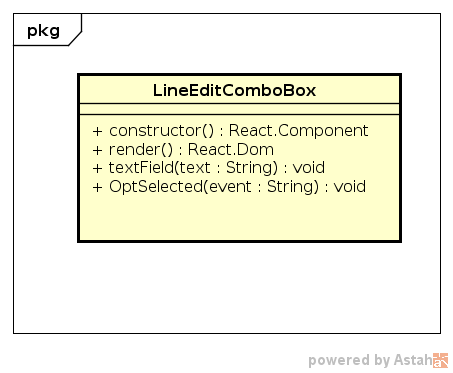
\includegraphics[width=0.6\textwidth]{img/single-LineEditComboBox}
   \caption{{Diagramma per LineEditComboBox in SingleComponents}}
\end{figure}
\FloatBarrier
\textbf{Descrizione}\\
Componente React che rappresenta una LineEdit con a fianco un ComboBox. \\\\
\\textbf{Metodi:} 
\\begin{itemize}

\\item +constructor(props : Object) : React.Component 
\\\\
Costruttore della sottoclasse di React.Component in cui è necessario chiamare super (props) ed è possibile inizializzare lo stato per i dati soggetti a cambiamento.

\\item +render() : React.DOM 
\\\\
Metodo che esamina this.props e this.state e restituisce un input di testo affiancato da una ComboBox.

\\end{itemize} 


\textbf{Applicazioni}\\
Componente React che unisce LineEdit e ComboBox.\\\\
Accetta le props per la costruzione dei due componenti interni e ne ritorna i risultati al "padre" tramite le props "textUpdate" e "comboUpdate". 


\clearpage

\subsubsection{RadioButtonGroup}
\textbf{Componente:}  Monolith::UI::SingleComponents\\
   \FloatBarrier
   \begin{figure}[ht]
   \centering
   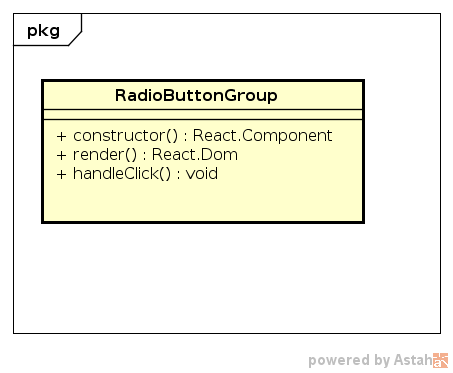
\includegraphics[width=0.6\textwidth]{img/single-RadioButtonGroup}
   \caption{{Diagramma per RadioButtonGroup in SingleComponents}}
\end{figure}
\FloatBarrier
\textbf{Descrizione}\\
Componente React che rappresenta un insieme di radio button tra cui è possibile scegliere tra opzioni mutualmente esclusive.\\\\

\\textbf{Metodi:} 
\\begin{itemize}
\\item +constructor(props : Object) : React.Component 
\\\\
Costruttore della sottoclasse di React.Component in cui è necessario chiamare super (props) ed è possibile inizializzare lo stato per i dati soggetti a cambiamento.

\\item +handleChange(event : Object): void 
\\\\
Viene passato al "padre" il valore selezionato.

\\item +render() : React.DOM 
\\\\
Metodo che esamina this.props e this.state e restituisce un gruppo di RadioButton con le opzioni che sono state date.

\\end{itemize} 


\textbf{Applicazioni}\\
Componente React che rappresenta un gruppo di RadioButton. \\\\ Le opzioni vengono passate con un array attraverso la props "options". 


\clearpage

\subsubsection{TextAreaComboBox}
\textbf{Componente:}  Monolith::UI::SingleComponents\\
   \FloatBarrier
   \begin{figure}[ht]
   \centering
   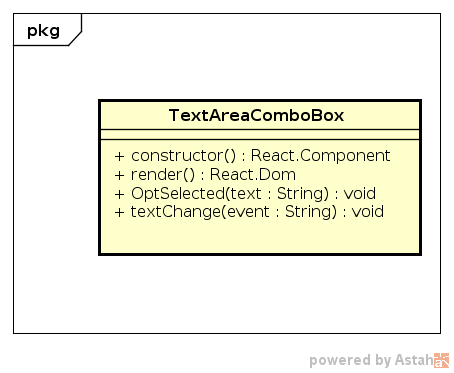
\includegraphics[width=0.6\textwidth]{img/single-TextAreaComboBox}
   \caption{{Diagramma per TextAreaComboBox in SingleComponents}}
\end{figure}
\FloatBarrier
\textbf{Descrizione}\\
Componente React che rappresenta una TextArea con a fianco un ComboBox \\\\
\\textbf{Metodi:} 
\\begin{itemize}

\\item +constructor(props : Object) : React.Component 
\\\\
Costruttore della sottoclasse di React.Component in cui è necessario chiamare super (props) ed è possibile inizializzare lo stato per i dati soggetti a cambiamento.

\\item +handleChange(event : String) : void  
\\\\ 
Comunica al "padre" il contenuto digitato nella textarea.

\\item +render() : React.DOM 
\\\\
Metodo che esamina this.props e this.state e restituisce un componente React composto da una textArea ed un ComboBox.

\\end{itemize} 


\textbf{Applicazioni}\\
Componente React che può essere utilizzato per la costruzione delle interfacce di alcune bolle.
\\\\ Vengono richieste anche le props per la costruzione dei degli elementi che formano il componente. 


\clearpage

\subsubsection{LineEditPushButton}
\textbf{Componente:}  Monolith::UI::SingleComponents\\
   \FloatBarrier
   \begin{figure}[ht]
   \centering
   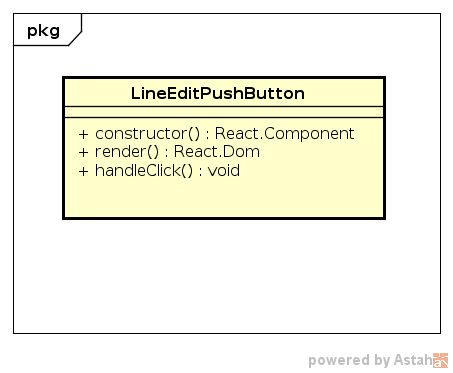
\includegraphics[width=0.6\textwidth]{img/single-LineEditPushButton}
   \caption{{Diagramma per LineEditPushButton in SingleComponents}}
\end{figure}
\FloatBarrier
\textbf{Descrizione}\\
Componente React che rappresenta un campo di inserimento testo affiancato ad un pulsante. \\\\
\\textbf{Metodi:} 
\\begin{itemize}

\\item +constructor(props : Object) : React.Component 
\\\\
Costruttore della sottoclasse di React.Component in cui è necessario chiamare super (props) ed è possibile inizializzare lo stato per i dati soggetti a cambiamento.

\\item +handleClick() : void  
\\\\
Passa al "padre" il testo contenuto nel LineEdit.

\\item ++textField() : void  
\\\\
Salva nello state il testo presente nel LineEdit.

\\item +render() : React.DOM 
\\\\
Metodo che esamina this.props e this.state e restituisce un componente React composto da un input di testo ed un pulsante di invio.

\\end{itemize} 


\textbf{Applicazioni}\\
Viene utilizzato per costruire alcune interfacce grafiche delle bolle.
Oltre alle props dei due componenti React, il componente si aspetta le seguenti props:
\\begin{itemize}

\\item classesle:
\\\\
Stile CSS per il LineEdit.
\\item classespb:
\\\\ 
Stile CSS per il PushButton.

\\item idle:
\\\\
ID per il LineEdit.
\\item idpb: 
\\\\
ID per il PushButton.
\\end{itemize} 


\clearpage

\subsubsection{AbsBubble}
\textbf{Componente:}  Monolith::UI::uiConstruction\\
   \FloatBarrier
   \begin{figure}[ht]
   \centering
   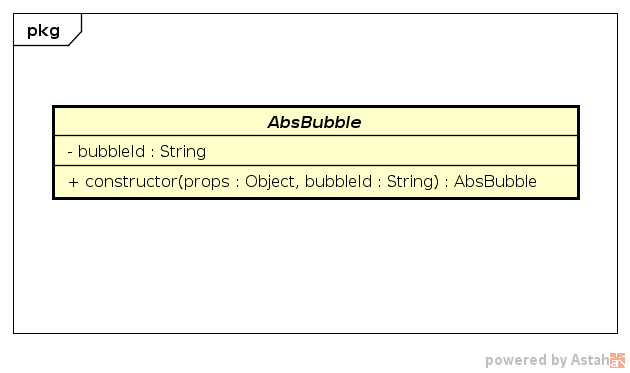
\includegraphics[width=0.6\textwidth]{img/single-AbsBubble}
   \caption{{Diagramma per AbsBubble in uiConstruction}}
\end{figure}
\FloatBarrier
\textbf{Descrizione}\\
Classe base astratta per le interfacce grafiche delle singole bolle. 


\textbf{Applicazioni}\\
Viene utilizzata come classe base da cui derivare le interfacce grafiche delle bolle. 


\clearpage

\subsubsection{AbsButton}
\textbf{Componente:}  Monolith::UI::uiConstruction\\
   \FloatBarrier
   \begin{figure}[ht]
   \centering
   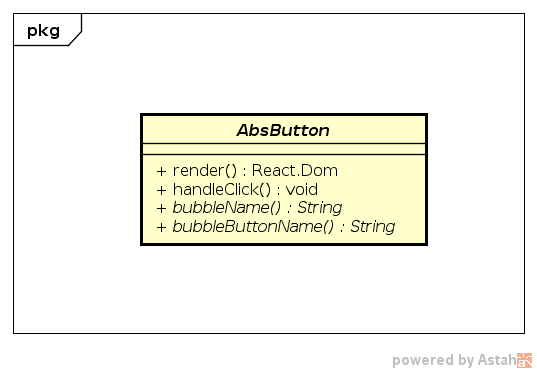
\includegraphics[width=0.6\textwidth]{img/single-AbsButton}
   \caption{{Diagramma per AbsButton in uiConstruction}}
\end{figure}
\FloatBarrier
\textbf{Descrizione}\\
Classe base dei pulsanti del menu di creazione delle nuove bolle. La classe base contiene molto codice e chiede classi derivate relativamente semplici. Viene usato il template pattern per parametrizzare gli aspetti che differiscono tra le classi derivate.
I seguenti metodi sono astratti puri:
\\begin{itemize}
\\item +bubbleName(): String \\\\
Nelle classi derivate ritorna il nome della bolla necessario per usare BubbleDiscriminator
\\item +bubbleButtonName(): String \\\\
Nelle classi derivate ritorna il testo che deve comparire nel pulsante
\\item +secondAreaName(): String \\\\
Nelle classi derivate ritorna il nome del componente React che deve essere inserito alla pressione del secondo pulsante. \\'E necessario per usare BubbleDiscriminator
\\end{itemize}
I seguenti metodi semplicemente eseguono le funzioni che vengono passate nelle props in risposta alla pressione dei pulsanti:
\\begin{itemize}
\\item +handleClick():void
\\item +handleSecondButton():void
\\end{itemize}
Il metodo render crea uno o due pulsanti a seconda che sia definito o meno il testo da inserire nel secondo pulsante nelle props. 


\textbf{Applicazioni}\\
Classe base da cui derivare per ottenere i pulsanti del menu di creazione di di nuove bolle 


\clearpage

\subsubsection{bubbleCreator}
\textbf{Componente:}  Monolith::UI::uiConstruction\\
   \FloatBarrier
   \begin{figure}[ht]
   \centering
   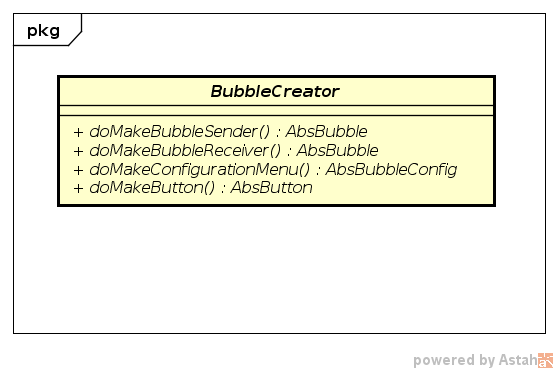
\includegraphics[width=0.6\textwidth]{img/single-bubbleCreator}
   \caption{{Diagramma per bubbleCreator in uiConstruction}}
\end{figure}
\FloatBarrier
\textbf{Descrizione}\\
Classe base astratta da cui poter derivare le classi concrete che si occupano della creazione delle istanze  di componenti grafici  \\\\ 
\\textbf{Metodi:}
\\begin{itemize}
\\item +doMakeBubbleSender() : ConcreteBubble 
\\\\
Ritorna il componente React per visualizzare una bolla inviata.
\\item +doMakeBubbleReceiver() : ConcreteBubble 
\\\\ 
Ritorna il componente React per visualizzare una bolla ricevuta.
\\item +doMakeConfigurationMenu() : ConcreteBubbleConfig 
\\\\
Ritorna il componente React per visualizzare il menù di creazione di una bolla da inviare.
\\item +doMakeButton() : ConcreteBubbleCreationButton 
\\\\ 
Ritorna il componente React per visualizzare il bottone di creazione del menù di configurazione di una bolla da inviare.

\\end{itemize} 


\textbf{Applicazioni}\\
Interfaccia che viene utilizzata come rappresentazione di concreteBubbleCreator. 


\clearpage

\subsubsection{AbsBubbleConfig}
\textbf{Componente:}  Monolith::UI::uiConstruction\\
   \FloatBarrier
   \begin{figure}[ht]
   \centering
   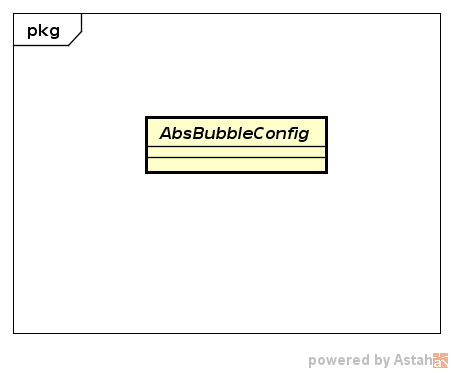
\includegraphics[width=0.6\textwidth]{img/single-AbsBubbleConfig}
   \caption{{Diagramma per AbsBubbleConfig in uiConstruction}}
\end{figure}
\FloatBarrier
\textbf{Descrizione}\\
Classe Astratta (interfaccia) per i menù di configurazione delle singole bolle. 


\textbf{Applicazioni}\\
Classe base da cui derivare per costruire i menù di configurazione delle bolle. 


\clearpage

\subsubsection{bubbleDiscriminator}
\textbf{Componente:}  Monolith::UI::uiConstruction\\
   \FloatBarrier
   \begin{figure}[ht]
   \centering
   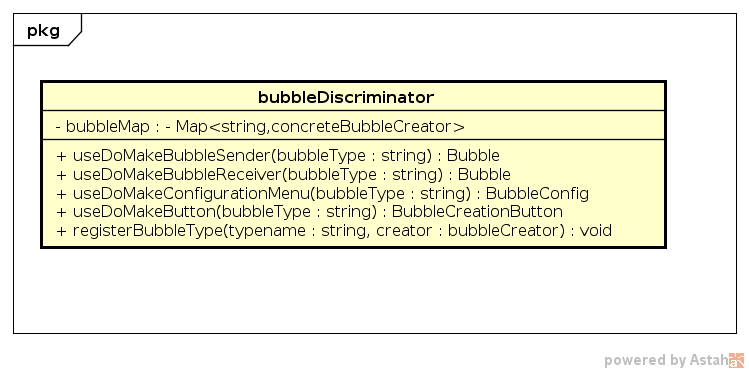
\includegraphics[width=0.6\textwidth]{img/single-bubbleDiscriminator}
   \caption{{Diagramma per bubbleDiscriminator in uiConstruction}}
\end{figure}
\FloatBarrier
\textbf{Descrizione}\\
Classe che contiene i metodi che ritornano le funzionalità necessarie per la rappresentazione delle bolle.

\\textbf{Attributi:}
\\begin{itemize}
\\item -bubbleMap : Map$<$string,concreteBubbleCreator$>$ 
\\\\
Struttura che mappa il nome di una bolla con l'istanza di concreteBubbleCreator per quella bolla.
\\end{itemize}
\\textbf{Metodi:} 
\\begin{itemize}
\\item +useDoMakeBubbleSender( bubbleType: string) : ConcreteBubble \\\\
Ritorna il componente React della stringa passata come parametro per visualizzare una bolla inviata.
\\item +useDoMakeBubbleReceiver( bubbleType: string) : ConcreteBubble \\\\
Ritorna il componente React della stringa passata come parametro per visualizzare una bolla ricevuta.
\\item +useDoMakeBubbleConfigurationMenu( bubbleType: string) : ConcreteBubbleConfig 
\\\\
Ritorna il componente React della stringa passata come parametro per visualizzare il menù di creazione di una bolla da inviare.
\\item  +useDoMakeButton( bubbleType: string) : ConcreteBubbleCreationButton \\\\
Ritorna il componente React della stringa passata come parametro per visualizzare il bottone di creazione del menù di configurazione di una bolla da inviare.

\\end{itemize} 


\textbf{Applicazioni}\\
Viene utilizzata quando si deve creare una nuova bolla, ritornando l'oggetto della bolla appena selezionata. 


\subsection{Architettura di dettaglio - Classi delle bolle demo}\subsubsection{CurrencyBubble}
\textbf{Componente:}  CurrencyBubble\\
   \FloatBarrier
   \begin{figure}[ht]
   \centering
   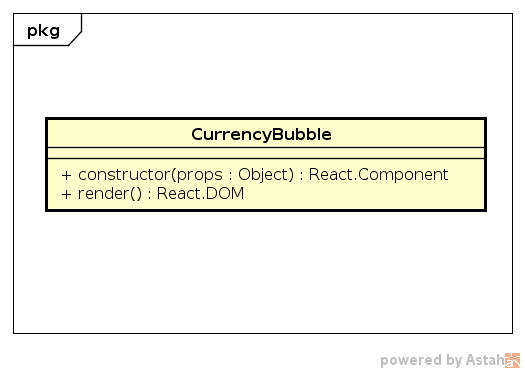
\includegraphics[width=0.6\textwidth]{img/single-CurrencyBubble}
   \caption{{Diagramma per CurrencyBubble in CurrencyBubble}}
\end{figure}
\FloatBarrier
\textbf{Descrizione}\\
Componente React che rappresenta l'interfaccia grafica di una CurrencyBubble
\\\\
\\textbf{Metodi:} 
\\begin{itemize}
\\item +constructor(props : Object) : React.Component 
\\\\
Costruttore della sottoclasse di React.Component in cui è necessario chiamare super (props) ed è possibile inizializzare lo stato per i dati soggetti a cambiamento.

\\item +render() : React.DOM 
\\\\
Metodo che esamina this.props e this.state e restituisce la CurrencyBubble a conversione avvenuta.

\\end{itemize} 


\textbf{Applicazioni}\\
Viene utilizzata per rappresentare graficamente la bolla di conversione valuta.
Il componente CurrencyBubble si aspetta in entrata le props contenetenti i dati di conversione: \\\\
\\begin{itemize}
\\item \\textit{curr_in}:
\\\\
Valore della valuta base.

\\item \\textit{curr_out}:
\\\\
Valore della valuta d'uscita.

\\item \\textit{value_in}:
\\\\
Valore di conversione iniziale.

\\item \\textit{value_out}:
\\\\
Valore finale di conversione.
\\end{itemize} 


\clearpage

\subsubsection{CurrencyCreator}
\textbf{Componente:}  CurrencyBubble\\
   \FloatBarrier
   \begin{figure}[ht]
   \centering
   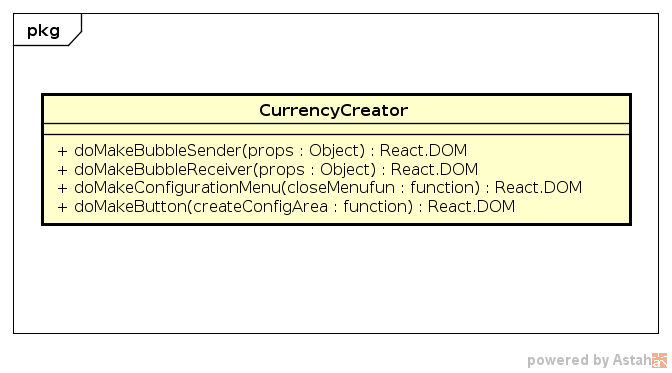
\includegraphics[width=0.6\textwidth]{img/single-CurrencyCreator}
   \caption{{Diagramma per CurrencyCreator in CurrencyBubble}}
\end{figure}
\FloatBarrier
\textbf{Descrizione}\\
Istanziazione concreta della classe Monolith::UI::Bubbles::BubbleCreator che gestisce la creazione della singola istanza di bolla convertitore di valuta, della singola istanza di menù di configurazione della bolla e della singola istanza di pulsante tramite l'utilizzo della classe Monolith::UI::Bubbles::BubbleDiscriminator.
\\\\
\\textbf{Metodi:} 
\\begin{itemize}
\\item +doMakeBubbleSender() : CurrencyBubble 
\\\\
Metodo che gestisce la creazione della bolla vista dal mittente.
\\item +doMakeBubbleReceiver() : CurrencyBubble 
\\\\
Metodo che gestisce la creazione della bolla vista dal ricevente.
\\item +doMakeConfigurationMenu() : CurrencyBubbleConfig 
\\\\
Metodo che gestisce la creazione dell'area di configurazione della bolla.
\\item +doMakeButton() : CurrencyBubbleCreationButton 
\\\\
Metodo che gestisce la creazione della singola istanza di pulsante da inserire nel menu iniziale di creazione. Viene lasciata l'implementazione della super classe.
\\end{itemize} 


\textbf{Applicazioni}\\
Viene utilizzata per gestire la creazione della singola istanza di bolla convertitore di valuta, della singola istanza di menù di configurazione della bolla e della singola istanza di pulsante. 


\clearpage

\subsubsection{CurrencyBubbleConfig}
\textbf{Componente:}  CurrencyBubble\\
   \FloatBarrier
   \begin{figure}[ht]
   \centering
   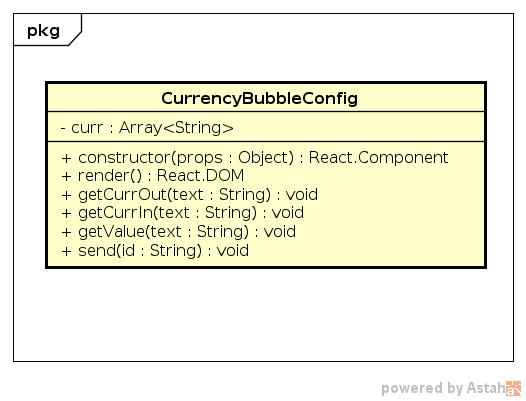
\includegraphics[width=0.6\textwidth]{img/single-CurrencyBubbleConfig}
   \caption{{Diagramma per CurrencyBubbleConfig in CurrencyBubble}}
\end{figure}
\FloatBarrier
\textbf{Descrizione}\\
Componente React che rappresenta il menù per la costruzione di una bolla di conversione valuta.
\\\\
\\textbf{Metodi:} 
\\begin{itemize}
\\item +constructor(props : Object) : React.Component 
\\\\
Costruttore della sottoclasse di React.Component in cui è necessario chiamare super (props) ed è possibile inizializzare lo stato per i dati di conversione e per quelli soggetti a cambiamento.

\\item +getCurrIn(text : String) : void 
\\\\
Salva la valuta di base.

\\item +getCurrOut(text : String) : void 
\\\\
Salva la valuta di uscita.

\\item +getValue(text : String) : void 
\\\\
Salva il valore iniziale di conversione.

\\item +send() : void 
\\\\
Salva i dati raccolti e li passa al "padre".

\\item +render() : React.DOM
\\\\
Metodo che esamina this.props e this.state, costruisce un array di opzioni modificabili e restituisce l'interfaccia grafica per il menù di creazione.
\\end{itemize} 


\textbf{Applicazioni}\\
Viene utilizzato per rappresentare il menù di configurazione della bolla di conversione valuta. Il componente React si aspetta, nella props "send", una funzioni che raccolga un oggetto contenente i dati della bolla. 


\clearpage

\subsubsection{CurrencyBubbleCreationButton}
\textbf{Componente:}  CurrencyBubble\\
   \FloatBarrier
   \begin{figure}[ht]
   \centering
   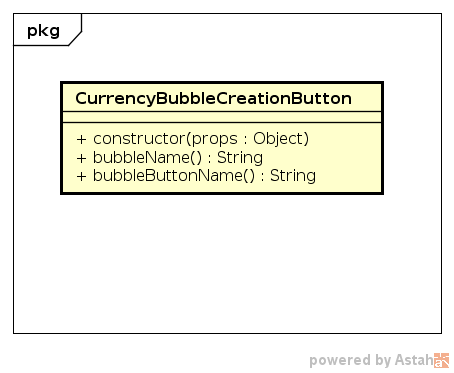
\includegraphics[width=0.6\textwidth]{img/single-CurrencyBubbleCreationButton}
   \caption{{Diagramma per CurrencyBubbleCreationButton in CurrencyBubble}}
\end{figure}
\FloatBarrier
\textbf{Descrizione}\\
Componente React che rappresenta il pulsante per creare una bolla di conversione valuta.
\\\\
\\textbf{Metodi:} 
\\begin{itemize}
\\item +constructor(props : Object) : React.Component 
\\\\
Costruttore della sottoclasse di React.Component in cui è necessario chiamare super (props) ed è possibile inizializzare lo stato per i dati soggetti a cambiamento.

\\item +bubbleButtonName() : String 
\\\\
Metodo che ritorna il nome presente sul pulsante.

\\item +bubbleName() : String 
\\\\
Metodo che ritorna il nome identificativo della bolla .

\\end{itemize} 


\textbf{Applicazioni}\\
Viene utilizzato per rappresentare il pulsante per la creazione di una bolla di conversione valuta.

Nella props "onClick" verrà ritornato il nome identificativo della bolla. 


\clearpage

\subsubsection{ListBubbleConfig}
\textbf{Componente:}  ListBubble::CheckListCreation\\
   \FloatBarrier
   \begin{figure}[ht]
   \centering
   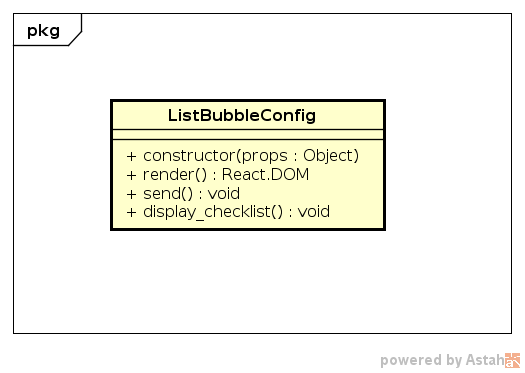
\includegraphics[width=0.6\textwidth]{img/single-ListBubbleConfig}
   \caption{{Diagramma per ListBubbleConfig in CheckListCreation}}
\end{figure}
\FloatBarrier
\textbf{Descrizione}\\
Componente React che rappresenta il menù per la costruzione di una bolla Lista.
\\\\
\\textbf{Metodi:} 
\\begin{itemize}
\\item +constructor(props : Object) : React.Component 
\\\\
Costruttore della sottoclasse di React.Component in cui è necessario chiamare super (props) ed è possibile inizializzare lo stato per i dati soggetti a cambiamento.

\\item +addOpt() : void 
\\\\
Aggiunge un campo opzione in più ad ogni click sul tasto apposito.

\\item +titleChange() : void 
\\\\
Salva il titolo che viene dato alla Lista.

\\item +optChange() : void 
\\\\
Salva il valore che viene dato ad ogni opzione.

\\item +send() : void 
\\\\
Salva i dati raccolti e li passa al "padre".

\\item +render() : React.DOM
\\\\
Metodo che esamina this.props e this.state, costruisce un array di opzioni modificabili e restituisce l'interfaccia grafica per il menù di creazione.
\\end{itemize} 


\textbf{Applicazioni}\\
Viene utilizzato per rappresentare il menù di configurazione della bolla Lista. Il componente React si aspetta, nella props "send", una funzione che raccolga un oggetto contenente i dati della bolla. 


\clearpage

\subsubsection{ListBubbleCreationButton}
\textbf{Componente:}  ListBubble::CheckListCreation\\
   \FloatBarrier
   \begin{figure}[ht]
   \centering
   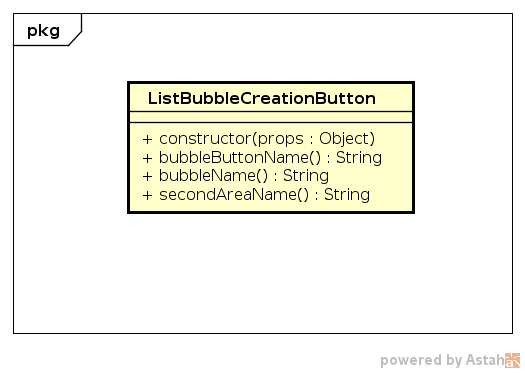
\includegraphics[width=0.6\textwidth]{img/single-ListBubbleCreationButton}
   \caption{{Diagramma per ListBubbleCreationButton in CheckListCreation}}
\end{figure}
\FloatBarrier
\textbf{Descrizione}\\
Componente React che rappresenta il pulsante per creare una bolla Lista.
\\\\
\\textbf{Metodi:} 
\\begin{itemize}
\\item +constructor(props : Object) : React.Component 
\\\\
Costruttore della sottoclasse di React.Component in cui è necessario chiamare super (props) ed è possibile inizializzare lo stato per i dati soggetti a cambiamento.

\\item +bubbleButtonName() : String 
\\\\
Metodo che ritorna il nome presente sul pulsante.

\\item +bubbleName() : String 
\\\\
Metodo che ritorna il nome identificativo della bolla .

\\end{itemize} 


\textbf{Applicazioni}\\
Viene utilizzato per rappresentare il pulsante per la creazione di una bolla Lista.

Nella props "onClick" verrà ritornato il nome identificativo della bolla. 


\clearpage

\subsubsection{ListBubble}
\textbf{Componente:}  ListBubble::CheckListReading\\
   \FloatBarrier
   \begin{figure}[ht]
   \centering
   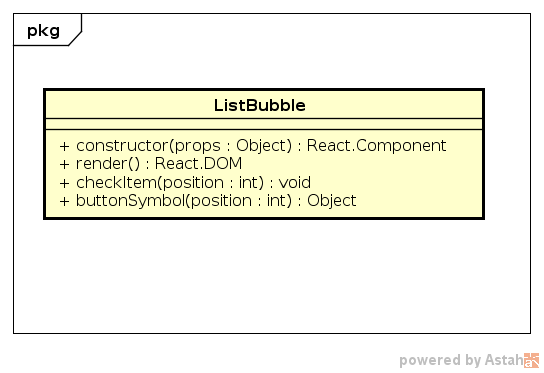
\includegraphics[width=0.6\textwidth]{img/single-ListBubble}
   \caption{{Diagramma per ListBubble in CheckListReading}}
\end{figure}
\FloatBarrier
\textbf{Descrizione}\\
Componente React che rappresenta l'interfaccia grafica di una ListBubble
\\\\
\\textbf{Metodi:} 
\\begin{itemize}
\\item +constructor(props : Object) : React.Component 
\\\\
Costruttore della sottoclasse di React.Component in cui è necessario chiamare super (props) ed è possibile inizializzare lo stato per i dati soggetti a cambiamento.

\\item +render() : React.DOM 
\\\\
Metodo che esamina this.props e this.state e restituisce elemento CheckBoxList 

\\item +changeCheck(m : Object) : void \\\\
Metodo che passa al "padre" i dati relativi alla checkbox cliccata.
\\end{itemize} 


\textbf{Applicazioni}\\
Viene utilizzata per rappresentare graficamente la bolla Lista.
Il componente ListBubble si aspetta in entrata una props "stat" che dovrà contenere un oggetto con i seguenti dati: \\\\
\\begin{itemize}
\\item \textit{op}:
\\\\
Un array di opzioni aventi un campo "id" ed un campo "value".
\\item \\textit{title}:
\\\\
Un titolo per la Lista.
\\end{itemize} 


\clearpage

\subsubsection{ListDb}
\textbf{Componente:}  ListBubble::Configuration\\
   \FloatBarrier
   \begin{figure}[ht]
   \centering
   \includegraphics[width=0.6\textwidth]{img/single-ListDb}
   \caption{{Diagramma per ListDb in Configuration}}
\end{figure}
\FloatBarrier
\textbf{Descrizione}\\
 


\textbf{Applicazioni}\\
 


\clearpage

\subsubsection{ListCheck}
\textbf{Componente:}  ListBubble::DataManagement\\
   \FloatBarrier
   \begin{figure}[ht]
   \centering
   \includegraphics[width=0.6\textwidth]{img/single-ListCheck}
   \caption{{Diagramma per ListCheck in DataManagement}}
\end{figure}
\FloatBarrier
\textbf{Descrizione}\\
 


\textbf{Applicazioni}\\
 


\clearpage

\subsubsection{ListBubbleCreator}
\textbf{Componente:}  ListBubble::DataManagement\\
   \FloatBarrier
   \begin{figure}[ht]
   \centering
   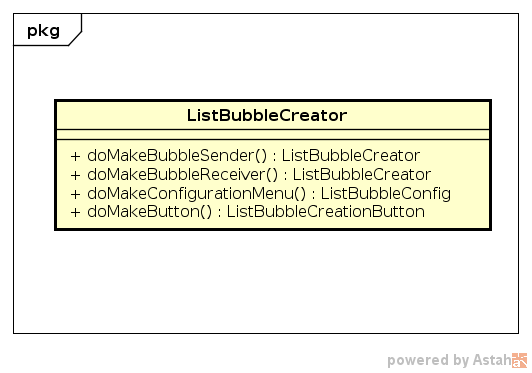
\includegraphics[width=0.6\textwidth]{img/single-ListBubbleCreator}
   \caption{{Diagramma per ListBubbleCreator in DataManagement}}
\end{figure}
\FloatBarrier
\textbf{Descrizione}\\
Istanziazione concreta della classe Monolith::UI::Bubbles::BubbleCreator che gestisce la creazione della singola istanza di bolla lista, della singola istanza di menù di configurazione della bolla e della singola istanza di pulsante tramite l'utilizzo della classe Monolith::UI::Bubbles::BubbleDiscriminator.
\\\\
\\textbf{Metodi:} 
\\begin{itemize}
\\item +doMakeBubbleSender() : ListBubble 
\\\\
Metodo che gestisce la creazione della bolla vista dal mittente.
\\item +doMakeBubbleReceiver() : ListBubble 
\\\\
Metodo che gestisce la creazione della bolla vista dal ricevente.
\\item +doMakeConfigurationMenu() : ListBubbleConfig 
\\\\
Metodo che gestisce la creazione dell'area di configurazione della bolla.
\\item +doMakeButton() : ListBubbleCreationButton 
\\\\
Metodo che gestisce la creazione dello specifico pulsante da inserire nel menu iniziale di creazione.
\\end{itemize} 


\textbf{Applicazioni}\\
Viene utilizzata per gestire la creazione della singola istanza di bolla lista, della singola istanza di menù di configurazione della bolla e della singola istanza di pulsante. 


\clearpage

\subsubsection{PollBubble}
\textbf{Componente:}  PollBubble\\
   \FloatBarrier
   \begin{figure}[ht]
   \centering
   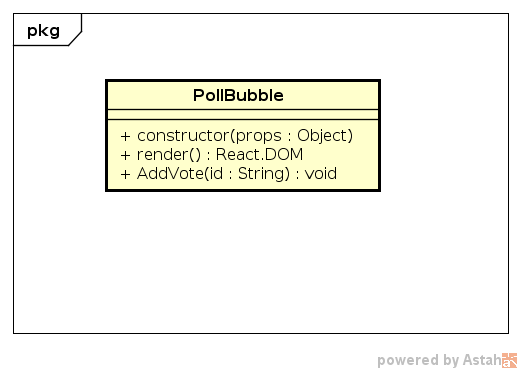
\includegraphics[width=0.6\textwidth]{img/single-PollBubble}
   \caption{{Diagramma per PollBubble in PollBubble}}
\end{figure}
\FloatBarrier
\textbf{Descrizione}\\
Componente React che rappresenta l'interfaccia grafica di una PollBubble
\\\\
\\textbf{Metodi:} 
\\begin{itemize}
\\item +constructor(props : Object) : React.Component 
\\\\
Costruttore della sottoclasse di React.Component in cui è necessario chiamare super (props) ed è possibile inizializzare lo stato per i dati soggetti a cambiamento.

\\item +render() : React.DOM 
\\\\
Metodo che esamina this.props e this.state e restituisce una lista di PushButton per votare il sondaggio. 

\\item +addVoto(id : String) : void \\\\
Metodo che da un voto all'opzione selezionata. Permette di votare una sola volta.

\\end{itemize} 


\textbf{Applicazioni}\\
Viene utilizzata per rappresentare graficamente la bolla Sondaggio.
Il componente PollBubble si aspetta in entrata i seguenti dati: \\\\
\\begin{itemize}
\\item \\textit{op}:
\\\\
Un array di opzioni.
\\item \\textit{title}:
\\\\
Un titolo per il sondaggio.
\\item \\textit{num}:
\\\\
Il numero delle opzioni.
\\item \\textit{id}:
\\\\
Un ID per la bolla Sondaggio.
\\end{itemize} 


\clearpage

\subsubsection{PollCreator}
\textbf{Componente:}  PollBubble\\
   \FloatBarrier
   \begin{figure}[ht]
   \centering
   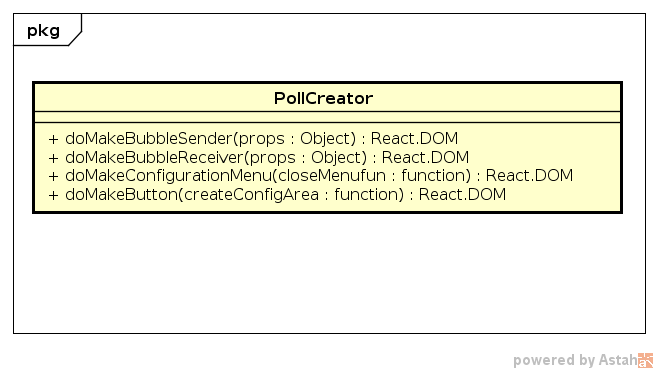
\includegraphics[width=0.6\textwidth]{img/single-PollCreator}
   \caption{{Diagramma per PollCreator in PollBubble}}
\end{figure}
\FloatBarrier
\textbf{Descrizione}\\
Istanziazione concreta della classe Monolith::UI::Bubbles::BubbleCreator che gestisce la creazione della singola istanza di bolla sondaggio, della singola istanza di menù di configurazione della bolla e della singola istanza di pulsante tramite l'utilizzo della classe Monolith::UI::Bubbles::BubbleDiscriminator.
\\\\
\\textbf{Metodi:} 
\\begin{itemize}
\\item +doMakeBubbleSender() : SurveyBubble 
\\\\
Metodo che gestisce la creazione della bolla vista dal mittente.
\\item +doMakeBubbleReceiver() : SurveyBubble 
\\\\
Metodo che gestisce la creazione della bolla vista dal ricevente.
\\item +doMakeConfigurationMenu() : SurveyBubbleConfig 
\\\\
Metodo che gestisce la creazione dell'area di configurazione della bolla.
\\item +doMakeButton() : SurveyBubbleCreationButton 
\\\\
Metodo che gestisce la creazione della singola istanza di pulsante da inserire nel menu iniziale di creazione. Viene lasciata l'implementazione della super classe.
\\end{itemize} 


\textbf{Applicazioni}\\
Viene utilizzata per gestire la creazione della singola istanza di bolla sondaggio, della singola istanza di menù di configurazione della bolla e della singola istanza di pulsante. 


\clearpage

\subsubsection{PollBubbleConfig}
\textbf{Componente:}  PollBubble\\
   \FloatBarrier
   \begin{figure}[ht]
   \centering
   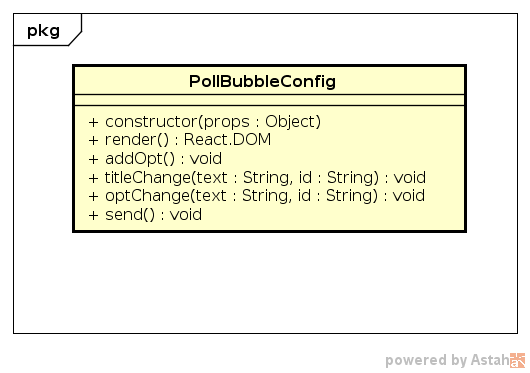
\includegraphics[width=0.6\textwidth]{img/single-PollBubbleConfig}
   \caption{{Diagramma per PollBubbleConfig in PollBubble}}
\end{figure}
\FloatBarrier
\textbf{Descrizione}\\
Componente React che rappresenta il menù per la costruzione di una bolla Sondaggio.
\\\\
\\textbf{Metodi:} 
\\begin{itemize}
\\item +constructor(props : Object) : React.Component 
\\\\
Costruttore della sottoclasse di React.Component in cui è necessario chiamare super (props) ed è possibile inizializzare lo stato per i dati soggetti a cambiamento.

\\item +addOpt() : void 
\\\\
Aggiunge un campo opzione in più ad ogni click sul tasto apposito.

\\item +titleChange() : void 
\\\\
Salva il titolo che viene dato alla Lista.

\\item +optChange() : void 
\\\\
Salva i valori che vengono dati ad ogni opzione.

\\item +send() : void 
\\\\
Salva i dati raccolti e li passa al "padre".

\\item +render() : React.DOM \\\\
Metodo che esamina this.props e this.state, costruisce un array di opzioni modificabili e restituisce l'interfaccia grafica per il menù di creazione.
\\end{itemize} 


\textbf{Applicazioni}\\
Viene utilizzato per rappresentare il menù di configurazione della bolla Sondaggio. Il componente React si aspetta, nella props "send", una funzione che raccolga un oggetto contenente i dati della bolla. 


\clearpage

\subsubsection{PollBubbleCreationButton}
\textbf{Componente:}  PollBubble\\
   \FloatBarrier
   \begin{figure}[ht]
   \centering
   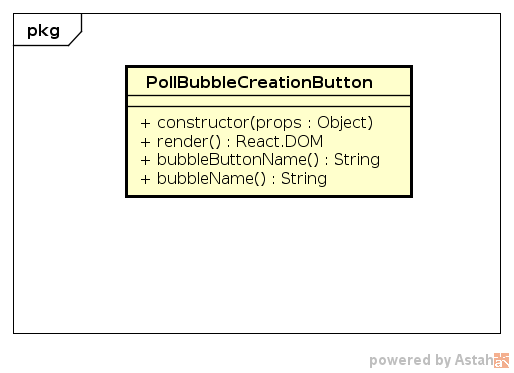
\includegraphics[width=0.6\textwidth]{img/single-PollBubbleCreationButton}
   \caption{{Diagramma per PollBubbleCreationButton in PollBubble}}
\end{figure}
\FloatBarrier
\textbf{Descrizione}\\
Componente React che rappresenta il pulsante per creare una bolla Sondaggio.
\\\\
\\textbf{Metodi:} 
\\begin{itemize}
\\item +constructor(props : Object) : React.Component 
\\\\
Costruttore della sottoclasse di React.Component in cui è necessario chiamare super (props) ed è possibile inizializzare lo stato per i dati soggetti a cambiamento.

\\item +bubbleButtonName() : String 
\\\\
Metodo che ritorna il nome presente sul pulsante.

\\item +bubbleName() : String 
\\\\
Metodo che ritorna il nome identificativo della bolla .

\\end{itemize} 


\textbf{Applicazioni}\\
Viene utilizzato per rappresentare il pulsante per la creazione di una bolla Sondaggio.

Nella props "onClick" verrà ritornato il nome identificativo della bolla. 


\clearpage

\subsubsection{RandBubble}
\textbf{Componente:}  RandomBubble\\
   \FloatBarrier
   \begin{figure}[ht]
   \centering
   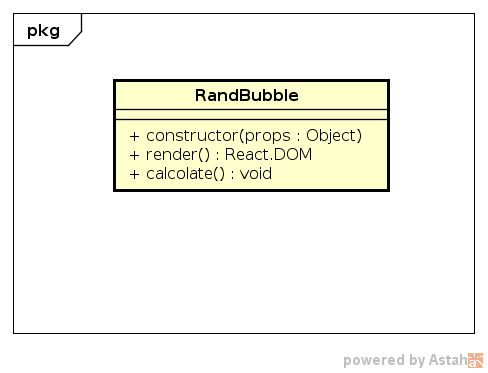
\includegraphics[width=0.6\textwidth]{img/single-RandBubble}
   \caption{{Diagramma per RandBubble in RandomBubble}}
\end{figure}
\FloatBarrier
\textbf{Descrizione}\\
Componente React che rappresenta l'interfaccia grafica di una RandBubble
\\\\
\\textbf{Metodi:} 
\\begin{itemize}
\\item +constructor(props : Object) : React.Component 
\\\\
Costruttore della sottoclasse di React.Component in cui è necessario chiamare super (props) ed è possibile inizializzare lo stato per i dati soggetti a cambiamento. 

\\item +render() : React.DOM 
\\\\
Metodo che esamina this.props e this.state e restituisce il numero random calcolato. 

\\item +calcolate() : void \\\\
Metodo che passa al "padre" il nuovo numero random estratto.
\\end{itemize} 


\textbf{Applicazioni}\\
Viene utilizzata per rappresentare graficamente la bolla Random.
Il componente RandBubble si aspetta in entrata una props "nMax" che dovrà contenere il numero delle facce del dado. 


\clearpage

\subsubsection{RandCreator}
\textbf{Componente:}  RandomBubble\\
   \FloatBarrier
   \begin{figure}[ht]
   \centering
   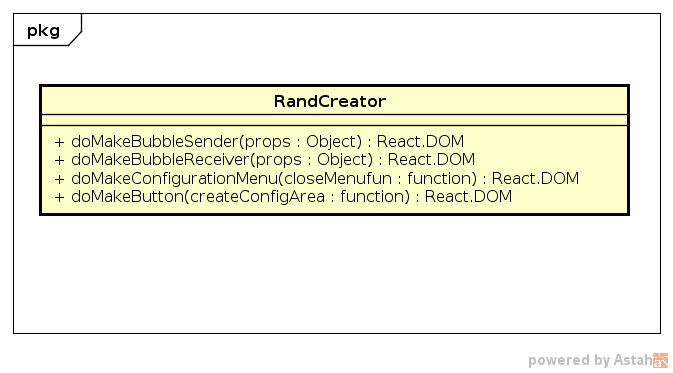
\includegraphics[width=0.6\textwidth]{img/single-RandCreator}
   \caption{{Diagramma per RandCreator in RandomBubble}}
\end{figure}
\FloatBarrier
\textbf{Descrizione}\\
Istanziazione concreta della classe Monolith::UI::Bubbles::BubbleCreator che gestisce la creazione della singola istanza di bolla estrazione di numero casuale, della singola istanza di menù di configurazione della bolla e della singola istanza di pulsante tramite l'utilizzo della classe Monolith::UI::Bubbles::BubbleDiscriminator.
\\\\
\\textbf{Metodi:} 
\\begin{itemize}
\\item +doMakeBubbleSender() : DiceBubble 
\\\\
Metodo che gestisce la creazione della bolla vista dal mittente.
\\item +doMakeBubbleReceiver() : DiceBubble 
\\\\
Metodo che gestisce la creazione della bolla vista dal ricevente.
\\item +doMakeConfigurationMenu() : DiceBubbleConfig 
\\\\
Metodo che gestisce la creazione dell'area di configurazione della bolla.
\\item +doMakeButton() : DiceBubbleCreationButton 
\\\\
Metodo che gestisce la creazione della singola istanza di pulsante da inserire nel menu iniziale di creazione. Viene lasciata l'implementazione della super classe.
\\end{itemize} 


\textbf{Applicazioni}\\
Viene utilizzata per gestire la creazione della singola istanza di bolla estrazione di numero casuale, della singola istanza di menù di configurazione della bolla e della singola istanza di pulsante. 


\clearpage

\subsubsection{RandBubbleConfig}
\textbf{Componente:}  RandomBubble\\
   \FloatBarrier
   \begin{figure}[ht]
   \centering
   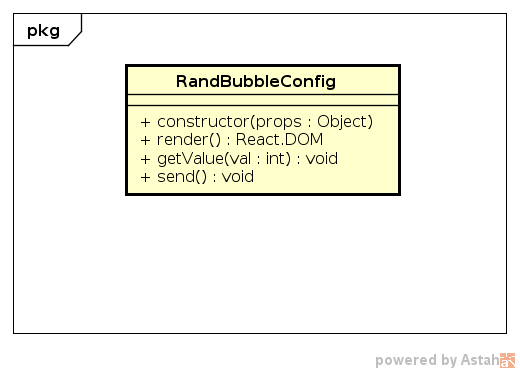
\includegraphics[width=0.6\textwidth]{img/single-RandBubbleConfig}
   \caption{{Diagramma per RandBubbleConfig in RandomBubble}}
\end{figure}
\FloatBarrier
\textbf{Descrizione}\\
Componente React che rappresenta il menù per la costruzione di una bolla di conversione valuta.
\\\\
\\textbf{Metodi:} 
\\begin{itemize}
\\item +constructor(props : Object) : React.Component 
\\\\
Costruttore della sottoclasse di React.Component in cui è necessario chiamare super (props) ed è possibile inizializzare lo stato per i dati soggetti a cambiamento.

\\item +getValue(val: String) : void 
\\\\
Salva il numero di facce del dado.

\\item +send() : void 
\\\\
Salva i dati raccolti e li passa al "padre".

\\item +render() : React.DOM \\\\
Metodo che esamina this.props e this.state e restituisce l'interfaccia grafica per il menù di creazione.
\\end{itemize} 


\textbf{Applicazioni}\\
Viene utilizzato per rappresentare il menù di configurazione della bolla di lancio casuale di dadi. Il componente React si aspetta, nella props "send", una funzioni che raccolga un oggetto contenente i dati della bolla. 


\clearpage

\subsubsection{RandBubbleCreationButton}
\textbf{Componente:}  RandomBubble\\
   \FloatBarrier
   \begin{figure}[ht]
   \centering
   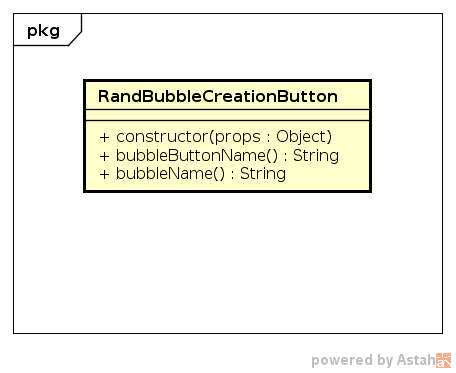
\includegraphics[width=0.6\textwidth]{img/single-RandBubbleCreationButton}
   \caption{{Diagramma per RandBubbleCreationButton in RandomBubble}}
\end{figure}
\FloatBarrier
\textbf{Descrizione}\\
Componente React che rappresenta il pulsante per creare una bolla di lancio casuale di dadi.
\\\\
\\textbf{Metodi:} 
\\begin{itemize}
\\item +constructor(props : Object) : React.Component 
\\\\
Costruttore della sottoclasse di React.Component in cui è necessario chiamare super (props) ed è possibile inizializzare lo stato per i dati soggetti a cambiamento.

\\item +bubbleButtonName() : String 
\\\\
Metodo che ritorna il nome presente sul pulsante.

\\item +bubbleName() : String 
\\\\
Metodo che ritorna il nome identificativo della bolla .

\\end{itemize} 


\textbf{Applicazioni}\\
Viene utilizzato per rappresentare il pulsante per la creazione di una bolla di lancio casuale di dadi.

Nella props "onClick" verrà ritornato il nome identificativo della bolla. 


